\documentclass{article}

\usepackage{amsmath} % math stuff
\usepackage{amssymb} % math stuff
\usepackage{array} % equations and stuff
\usepackage{bm} % bold math
%\usepackage{booktabs} % extra table rule options
%\usepackage{caption} % suppressed table numbering; incompatible with revtex, and longtable, I think
\usepackage{comment} % comment environment
%\usepackage{enumitem} % customization of enumeration, itemize, and description
\usepackage[T1]{fontenc} % font encoding for special characters, must also use scalable font package
\usepackage[margin=0.8in]{geometry} % paper sizes and margins (but be careful not to mess up pre-defined pages)
\usepackage{graphicx} % for graphics
%\usepackage{helvet} % default font is the helvetica postscript font
\usepackage{layouts} % print units like widths
\usepackage{lipsum} % lorem ipsum filler text
\usepackage{lmodern} % scalable font?
\usepackage{longtable} % multi-page tables
\usepackage{makecell} % specify line-breaks in table cells
\usepackage{mathrsfs} % math script font
\usepackage{mhchem} % easier chemical formula
\usepackage{microtype} % allows disabling of ligatures
%\usepackage{newcent} % new century schoolbook font
\usepackage{nicefrac}
\usepackage{numprint} % print and format (large) numbers
\usepackage{parskip} % removes paragraph indentation, and adjusts paragraph skip, as well as list items
\usepackage{pdfpages} % add pdf files as pages
%\usepackage{setspace} % adjust text spacing and indents
\usepackage{siunitx} % decimal alignment
\usepackage{subfigure} % divided figures
%\usepackage{tabu} % extra table options
\usepackage{textcomp} % symbols
\usepackage{threeparttablex} % better footnotes with longtable
\usepackage{titling} % title placement
\usepackage{ulem} % strikethrough text
%\usepackage{url} % superceded by hyperref
\usepackage{verbatim} % verbatim environment
\usepackage{xcolor} % colors and color boxes
\usepackage{xspace} % commands that don't eat up white space
\usepackage{hyperref} % links and page setup; should always come last

\hypersetup{
 bookmarks=true,
 colorlinks=true,
 citecolor=blue,
 linkcolor=blue,
 urlcolor=blue,
 pdfstartview={XYZ null null 1.0} % default open view is 100%
}

\DisableLigatures[f,t]{encoding = T1} % disable ff, fi, fl, tt ligatures; without options, it also disables -- = endash
\renewcommand{\arraystretch}{1.0} % extra vertical (and horizontal?) space in tables

% define centered, left- and right-aligned columns with specified widths
\newcommand{\PreserveBackslash}[1]{\let\temp=\\#1\let\\=\temp}
\newcolumntype{C}[1]{>{\PreserveBackslash\centering}p{#1}}
\newcolumntype{L}[1]{>{\PreserveBackslash\raggedright}p{#1}}
\newcolumntype{R}[1]{>{\PreserveBackslash\raggedleft}p{#1}}

\begin{document}

\pagestyle{empty} % don't number pages

% custom title
\begin{center}
{\LARGE Express Riddler}

\vspace{0.15in}

{\Large 7 May 2021}
\end{center}


\section*{Riddle:}

Martina and Olivia each secretly generate their own random real number, selected uniformly between 0 and 1.
Starting with Martina, they take turns declaring (so the other can hear) who they think probably has the greater number until the first moment they agree.
Throughout this process, their respective numbers do not change.
So for example, their dialogue might go as follows:

Martina: My number is probably bigger.

Olivia: My number is probably bigger.

Martina: My number is probably bigger.

Olivia: My number is probably bigger.

Martina: Olivia's number is probably bigger.

They are playing as a team, hoping to maximize the chances they correctly predict who has the greater number.

For any given round with randomly generated numbers, what is the probability that the person they agree on really does have the bigger number?

\textit{Extra credit}: Martina and Olivia change the rules so that they stop when Olivia first says that she agrees with Martina.
That is, if Martina says on her turn that she agrees with Olivia, that is not a condition for stopping.
Again, if they play to maximizing their chances, what is the probability that the person they agree on really does have the bigger number?



\section*{Solution:}

If the numbers for Martina and Olivia are labeled $x$ and $y$, respectively, then the possible pairs of numbers $(x,y)$ are spread evenly across a unit square.
The square is divided in half by the line $y=x$, with the bottom/right half representing Martina's number being larger, and the upper/left half representing Olivia's number being larger.
Because the numbers chosen uniformly from the reals, the probability that the numbers are the same is 0.
(I am also assuming that the generated numbers are independent; this seems to be implied, though not explicitly stated.)

Once Martina makes her first declaration (for example, that hers is probably bigger), the distribution of numbers is reduced from a square to a rectangle, of width \nicefrac{1}{2}, and height 1.
Martina's statement is equivalent to saying that her number is either less than or greater than \nicefrac{1}{2}.
Again, because they are real numbers, the probability of her number being exactly \nicefrac{1}{2} is 0.
From here on, each statement of disagreement (my number is probably bigger) reduces the size of the rectangle by a factor of 4.
Martina's first statement creates a division across \nicefrac{1}{2}.
If Olivia's number is also in the same range (less than or greater than \nicefrac{1}{2}), she must determine if her number is in the upper half or lower half of this range.
If it is in the upper half (greater than \nicefrac{3}{4}), she disagrees, and creates a new rectangle with width \nicefrac{1}{2} and height \nicefrac{1}{4}.
On the other hand, if Olivia's number is less than \nicefrac{3}{4}, she will make a statement of agreement (further, if her number is less than \nicefrac{1}{2}, her statement has certainty).
Each disgreement in sequence similarly reduces the rectangle, moving the rectangle to the extremes of the unit square.
Importantly, each statement of disagreement does not change the shape of the rectangle, nor does it change the position of the rectangle relative to the line $y=x$.

In the fastest case, Olivia would agree on her first opportunity.
This is illustrated below.
Martina's number is greater than \nicefrac{1}{2}, and Olivia's is less than \nicefrac{3}{4}.
The resulting rectangle of possible values is shown by the combination of green and red regions.
The green region (labeled A) is below/right of the dividing line $y=x$, and shows the space where Martina and Olivia are correct.
The red region (B) is above/left of the dividing line, and shows where they are incorrect.
The probability of them being right is simply the relative area of region A.
Doing some simple geometry leads to an answer of \nicefrac{A}{(A+B)}=\nicefrac{11}{12}.

\begin{center}
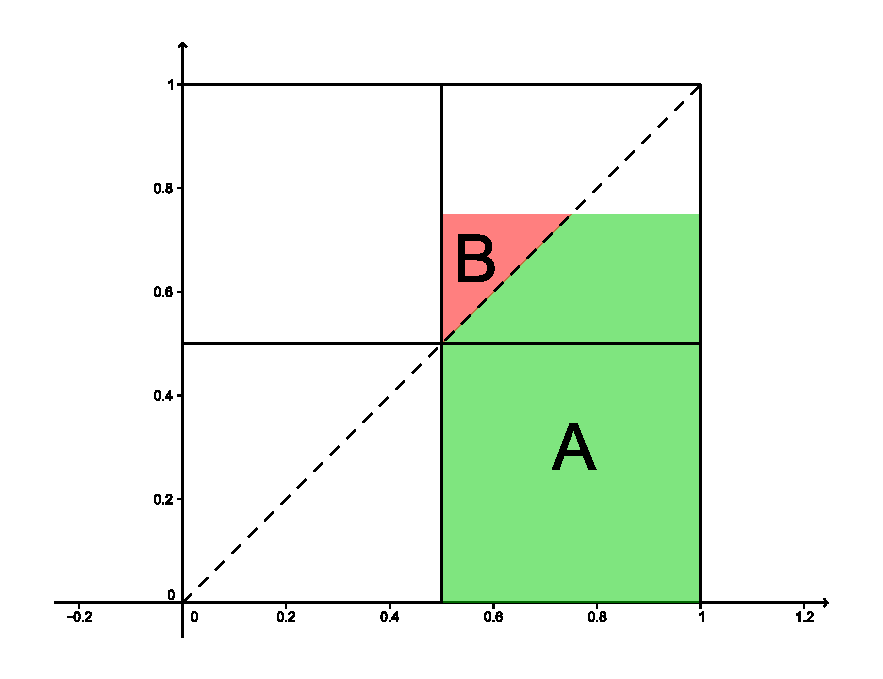
\includegraphics[width=4in]{Grid.pdf}
\end{center}
\vspace{0.1in}

Because any subsequent agreement produces a similar rectangle, the answer is the same for any sequence of statements.
So the solution to the riddle is
\fcolorbox{red}{white}{\bf\nicefrac{11}{12}}\,.


Alternately, the entire unit square can be filled in, and the complete green and red areas can be solved.
The graph I made illustrates the case that Martina's number is greater than \nicefrac{1}{2}.
The case with her number less than \nicefrac{1}{2} also creates the same size rectangle, but rotated across the center of the unit square.
Every other possible sequence of statements (starting either greater or less than \nicefrac{1}{2}) results in rectangles that get smaller by a factor of 4 and fill in the upper right and bottom left corners piece by piece.
These create a geometric series of regions, and summing up the infinite regions gives the complete result:

\begin{align*}
\textrm{Green}&=2\cdot\sum_{i=0}^{\infty}\textrm{A}\left(\frac{1}{4}\right)^{i} \\
              &=2\cdot\frac{11}{32}\cdot\sum_{i=0}^{\infty}\left(\frac{1}{4}\right)^{i} \\
              &=\frac{11}{16}\cdot\frac{1}{1-\nicefrac{1}{4}} \\
              &=\frac{11}{16}\cdot\frac{4}{3} \\
              &=\frac{11}{12}
\end{align*}



\end{document}